\documentclass [a4paper] {article}

\usepackage[dvipsnames]{xcolor}

\usepackage{fancyvrb}

\RecustomVerbatimCommand{\VerbatimInput}{VerbatimInput}
{fontsize=\footnotesize,frame=lines,framesep=2em,rulecolor=\color{Gray},commandchars=\|\(\),commentchar=*}

\title{R-PL1}
\author{Gabriel L\'opez, Sergio Sanz, \'Alvaro Zamorano}

\usepackage{Sweave}
\begin{document}

\maketitle

En esta parte de la pr\'actica trabajaremos con el fichero
\texttt{satelites.txt}.\\

\bigskip
En primer lugar hay que leer este fichero, para ello usamos
la funci\'on:
\begin{Schunk}
\begin{Sinput}
> satelites<-read.table("satelites.txt")
\end{Sinput}
\end{Schunk}

\bigskip
Para trabajar con la variable radio, y hacer este trabajo m\'as
c\'omodo, la cargamos en una variable:
\begin{Schunk}
\begin{Sinput}
> Radio<-satelites$Radio
\end{Sinput}
\end{Schunk}

\bigskip
En el primer an\'alisis de los datos se cuantifica la \textbf{frecuencia}
de aparici\'on de los mismos. 

%%%%%%%%%%%%%%%%%%%%%%%%%%%%%%%%%%%%%%%%%%

\graphicspath{ {C:/Users/tromp/Documents/1.Curso_2019-20/1.Cuatrimetestre/2.Ciencia_Datos/LAB/CienciaDatos/Practica1/} }

\begin{enumerate}
\item
\textit{Frecuencia absoluta: }
\begin{Schunk}
\begin{Sinput}
> frabsradio<-table(Radio)
> write.table(frabsradio, "C:/Users/tromp/Documents/1.Curso_2019-20/1.Cuatrimetestre/2.Ciencia_Datos/LAB/CienciaDatos/Practica1/p.txt", sep="\t", row.names=F) 
> 
\end{Sinput}
\end{Schunk}

\VerbatimInput{p.txt}

%
\includegraphics[width=\textwidth]{frabsradio}

%%%%%%%%%%%%%%%%%%%%%%%%%%%%%%%%%%%%%%%%%

\item
\textit{Frecuencia absoluta acumulada: }
\begin{Schunk}
\begin{Sinput}
> frabsacumradio<-cumsum(table(Radio))
> frabsacumradio
\end{Sinput}
\begin{Soutput}
13 15 16 20 22 27 29 30 33 34 42 
 1  2  3  5  6  7  8  9 10 11 12 
\end{Soutput}
\end{Schunk}

\item
\textit{Frecuencia relativa: }En este caso es necesario crear una funci\'on
para poder calcular este valor. La funci\'on es:
\begin{Schunk}
\begin{Sinput}
> frecrel<-function(Radio){table(Radio)/length(Radio)}
> frecrel(Radio)
\end{Sinput}
\begin{Soutput}
Radio
        13         15         16         20         22         27         29         30         33         34         42 
0.08333333 0.08333333 0.08333333 0.16666667 0.08333333 0.08333333 0.08333333 0.08333333 0.08333333 0.08333333 0.08333333 
\end{Soutput}
\end{Schunk}

\item
\textit{Frecuencia relativa acumulada: }Haremos uso de la funci\'on definida anteriormente:
\begin{Schunk}
\begin{Sinput}
> frecrelacum<-function(Radio){cumsum(table(Radio)/length(Radio))}
> frecrelacum(Radio)
\end{Sinput}
\begin{Soutput}
        13         15         16         20         22         27         29         30         33         34         42 
0.08333333 0.16666667 0.25000000 0.41666667 0.50000000 0.58333333 0.66666667 0.75000000 0.83333333 0.91666667 1.00000000 
\end{Soutput}
\end{Schunk}
\end{enumerate}

\bigskip
El segundo an\'alisis de los datos se basa en calcular la \textbf{media aritm\'etica:}
\begin{Schunk}
\begin{Sinput}
> mr=mean(Radio)
> mr
\end{Sinput}
\begin{Soutput}
[1] 25.08333
\end{Soutput}
\end{Schunk}

\bigskip
El tercer an\'alisis de los datos se basa en calcular las \textbf{medidas de dispersi\'on:}
\begin{enumerate}
\item
\textit{Desviaci\'on t\'ipica: }Para corregir los resultados, se hace el c\'alculo
a trav\'es de:
\begin{Schunk}
\begin{Sinput}
> sdr<-sd(Radio)/sqrt(12/11)
> sdr
\end{Sinput}
\begin{Soutput}
[1] 8.47996
\end{Soutput}
\end{Schunk}

\item
\textit{Varianza: }Al igual que en el caso anterior es necesario corregir el 
resultado por lo que se usa:
\begin{Schunk}
\begin{Sinput}
> varr<-var(Radio)*11/12
> varr
\end{Sinput}
\begin{Soutput}
[1] 71.90972
\end{Soutput}
\end{Schunk}
\end{enumerate}

\bigskip
El cuarto an\'alisis de los datos se basa en las \textbf{medidas de ordenaci\'on,} antes de los c\'alculos es necesario ordenar
los datos en funci\'on de la variable usada, en este caso el radio.
\begin{Schunk}
\begin{Sinput}
> so<-satelites[order(Radio),]
\end{Sinput}
\end{Schunk}

\bigskip
Realmente no ser\'ia necesario ordenar los datos, ya que R se encarga de ello
en caso de no hacerlo. Se procede a realizar los c\'alculos:

\begin{enumerate}
\item
\textit{Mediana:}
\begin{Schunk}
\begin{Sinput}
> mediant<-median(Radio)
> mediant
\end{Sinput}
\begin{Soutput}
[1] 24.5
\end{Soutput}
\end{Schunk}

\item
\textit{Cuartiles:}
\begin{Schunk}
\begin{Sinput}
> cuar1<-quantile(Radio,0.25)
> cuar1
\end{Sinput}
\begin{Soutput}
25% 
 19 
\end{Soutput}
\begin{Sinput}
> cuar2<-quantile(Radio,0.5)
> cuar2
\end{Sinput}
\begin{Soutput}
 50% 
24.5 
\end{Soutput}
\begin{Sinput}
> cuar3<-quantile(Radio,0.75)
> cuar3
\end{Sinput}
\begin{Soutput}
  75% 
30.75 
\end{Soutput}
\begin{Sinput}
> cuar54<-quantile(Radio,0.54)
> cuar54
\end{Sinput}
\begin{Soutput}
 54% 
26.7 
\end{Soutput}
\end{Schunk}
\end{enumerate}

%%%%%%%%%%%%%%%%%%%%%%%%%%%%%%%%%%%%%%%%%%%%%%%%%%%%%%%%%%%%%%%%%%%%%%%%%%%%%%%%%%%%%%%%%%%%%%%%%%%%%%%%%%%%%%%%%%%%%%%%%%%%%%%
\bigskip
A continuaci\'on pasaremos a trabajar con un fichero generado por SPSS, 
\texttt{cardata.sav}.\\

\bigskip
En primer lugar hay que leer este fichero pero no disponemos de la librer\'ia
necesaria para hacerlo, para cargarla usamos:
\begin{Schunk}
\begin{Sinput}
> library(foreign)
\end{Sinput}
\end{Schunk}
Esta librer\'ia se trata de una librer\'ia est\'andar de R.

\bigskip
Una vez cargada procedemos a su lectura
\begin{Schunk}
\begin{Sinput}
> A<-read.spss("cardata.sav")
\end{Sinput}
\end{Schunk}

\bigskip
Para trabajar con la variable mpg, y hacer este trabajo m\'as
c\'omodo, la cargamos en una variable:
\begin{Schunk}
\begin{Sinput}
> mpg<-A$mpg
\end{Sinput}
\end{Schunk}

\bigskip
La variable mpg contiene valores NA, es decir, valores que no se encuentran disponibles 
por lo que es imposible realizar c\'alculos con ella. Para eliminar estos valores usamos:
\begin{Schunk}
\begin{Sinput}
> mpg<-mpg[!is.na(mpg)]
\end{Sinput}
\end{Schunk}

\bigskip
En el primer an\'alisis de los datos se cuantifica la \textbf{frecuencia}
de aparici\'on de los mismos. 

\begin{enumerate}
\item
\textit{Frecuencia absoluta: }
\begin{Schunk}
\begin{Sinput}
> frabsmpg<-table(mpg)
> frabsmpg
\end{Sinput}
\begin{Soutput}
mpg
15.5 16.2 16.5 16.9   17 17.5 17.6 17.7 18.1 18.2 18.5 18.6 19.1 19.2 19.4 19.8 19.9 20.2 20.3 20.5 20.6 20.8 21.1 21.5 21.6   22 22.3 22.4   23 23.2 23.5 23.6 23.7 
   1    1    1    1    2    1    2    1    2    1    1    1    1    3    2    1    1    4    1    2    2    1    1    1    1    1    1    1    2    1    1    1    1 
23.8 23.9   24 24.2 24.3   25 25.1 25.4 25.8   26 26.4 26.6 26.8   27 27.2 27.4 27.5 27.9   28 28.1 28.4 28.8   29 29.5 29.8 29.9   30 30.4 30.7 30.9   31 31.3 31.5 
   1    2    1    1    1    1    1    2    1    1    1    2    1    4    3    1    1    1    3    1    1    1    1    1    2    1    2    1    1    1    3    1    1 
31.6 31.8 31.9   32 32.1 32.2 32.3 32.4 32.7 32.8 32.9   33 33.5 33.7 33.8   34 34.1 34.2 34.3 34.4 34.5 34.7   35 35.1 35.7   36 36.1 36.4   37 37.2 37.3 37.7   38 
   1    1    1    3    1    1    1    2    1    1    1    1    1    1    1    2    2    1    1    1    2    1    1    1    1    5    2    1    3    1    1    1    4 
38.1   39 39.1 39.4 40.8 40.9 41.5 43.1 43.4   44 44.3 44.6 46.6 
   1    1    1    1    1    1    1    1    1    1    1    1    1 
\end{Soutput}
\end{Schunk}

\item
\textit{Frecuencia absoluta acumulada: }
\begin{Schunk}
\begin{Sinput}
> frabsacummpg<-cumsum(table(mpg))
> frabsacummpg
\end{Sinput}
\begin{Soutput}
15.5 16.2 16.5 16.9   17 17.5 17.6 17.7 18.1 18.2 18.5 18.6 19.1 19.2 19.4 19.8 19.9 20.2 20.3 20.5 20.6 20.8 21.1 21.5 21.6   22 22.3 22.4   23 23.2 23.5 23.6 23.7 
   1    2    3    4    6    7    9   10   12   13   14   15   16   19   21   22   23   27   28   30   32   33   34   35   36   37   38   39   41   42   43   44   45 
23.8 23.9   24 24.2 24.3   25 25.1 25.4 25.8   26 26.4 26.6 26.8   27 27.2 27.4 27.5 27.9   28 28.1 28.4 28.8   29 29.5 29.8 29.9   30 30.4 30.7 30.9   31 31.3 31.5 
  46   48   49   50   51   52   53   55   56   57   58   60   61   65   68   69   70   71   74   75   76   77   78   79   81   82   84   85   86   87   90   91   92 
31.6 31.8 31.9   32 32.1 32.2 32.3 32.4 32.7 32.8 32.9   33 33.5 33.7 33.8   34 34.1 34.2 34.3 34.4 34.5 34.7   35 35.1 35.7   36 36.1 36.4   37 37.2 37.3 37.7   38 
  93   94   95   98   99  100  101  103  104  105  106  107  108  109  110  112  114  115  116  117  119  120  121  122  123  128  130  131  134  135  136  137  141 
38.1   39 39.1 39.4 40.8 40.9 41.5 43.1 43.4   44 44.3 44.6 46.6 
 142  143  144  145  146  147  148  149  150  151  152  153  154 
\end{Soutput}
\end{Schunk}

\item
\textit{Frecuencia relativa: }En este caso es necesario crear una funci\'on
para poder calcular este valor. La funci\'on es:
\begin{Schunk}
\begin{Sinput}
> frecrel<-function(mpg){table(mpg)/length(mpg)}
> frecrel(mpg)
\end{Sinput}
\begin{Soutput}
mpg
       15.5        16.2        16.5        16.9          17        17.5        17.6        17.7        18.1        18.2        18.5        18.6        19.1 
0.006493506 0.006493506 0.006493506 0.006493506 0.012987013 0.006493506 0.012987013 0.006493506 0.012987013 0.006493506 0.006493506 0.006493506 0.006493506 
       19.2        19.4        19.8        19.9        20.2        20.3        20.5        20.6        20.8        21.1        21.5        21.6          22 
0.019480519 0.012987013 0.006493506 0.006493506 0.025974026 0.006493506 0.012987013 0.012987013 0.006493506 0.006493506 0.006493506 0.006493506 0.006493506 
       22.3        22.4          23        23.2        23.5        23.6        23.7        23.8        23.9          24        24.2        24.3          25 
0.006493506 0.006493506 0.012987013 0.006493506 0.006493506 0.006493506 0.006493506 0.006493506 0.012987013 0.006493506 0.006493506 0.006493506 0.006493506 
       25.1        25.4        25.8          26        26.4        26.6        26.8          27        27.2        27.4        27.5        27.9          28 
0.006493506 0.012987013 0.006493506 0.006493506 0.006493506 0.012987013 0.006493506 0.025974026 0.019480519 0.006493506 0.006493506 0.006493506 0.019480519 
       28.1        28.4        28.8          29        29.5        29.8        29.9          30        30.4        30.7        30.9          31        31.3 
0.006493506 0.006493506 0.006493506 0.006493506 0.006493506 0.012987013 0.006493506 0.012987013 0.006493506 0.006493506 0.006493506 0.019480519 0.006493506 
       31.5        31.6        31.8        31.9          32        32.1        32.2        32.3        32.4        32.7        32.8        32.9          33 
0.006493506 0.006493506 0.006493506 0.006493506 0.019480519 0.006493506 0.006493506 0.006493506 0.012987013 0.006493506 0.006493506 0.006493506 0.006493506 
       33.5        33.7        33.8          34        34.1        34.2        34.3        34.4        34.5        34.7          35        35.1        35.7 
0.006493506 0.006493506 0.006493506 0.012987013 0.012987013 0.006493506 0.006493506 0.006493506 0.012987013 0.006493506 0.006493506 0.006493506 0.006493506 
         36        36.1        36.4          37        37.2        37.3        37.7          38        38.1          39        39.1        39.4        40.8 
0.032467532 0.012987013 0.006493506 0.019480519 0.006493506 0.006493506 0.006493506 0.025974026 0.006493506 0.006493506 0.006493506 0.006493506 0.006493506 
       40.9        41.5        43.1        43.4          44        44.3        44.6        46.6 
0.006493506 0.006493506 0.006493506 0.006493506 0.006493506 0.006493506 0.006493506 0.006493506 
\end{Soutput}
\end{Schunk}

\item
\textit{Frecuencia relativa acumulada: }Haremos uso de la funci\'on definida anteriormente:
\begin{Schunk}
\begin{Sinput}
> frecrelacum<-function(mpg){cumsum(table(mpg)/length(mpg))}
> frecrelacum(mpg)
\end{Sinput}
\begin{Soutput}
       15.5        16.2        16.5        16.9          17        17.5        17.6        17.7        18.1        18.2        18.5        18.6        19.1 
0.006493506 0.012987013 0.019480519 0.025974026 0.038961039 0.045454545 0.058441558 0.064935065 0.077922078 0.084415584 0.090909091 0.097402597 0.103896104 
       19.2        19.4        19.8        19.9        20.2        20.3        20.5        20.6        20.8        21.1        21.5        21.6          22 
0.123376623 0.136363636 0.142857143 0.149350649 0.175324675 0.181818182 0.194805195 0.207792208 0.214285714 0.220779221 0.227272727 0.233766234 0.240259740 
       22.3        22.4          23        23.2        23.5        23.6        23.7        23.8        23.9          24        24.2        24.3          25 
0.246753247 0.253246753 0.266233766 0.272727273 0.279220779 0.285714286 0.292207792 0.298701299 0.311688312 0.318181818 0.324675325 0.331168831 0.337662338 
       25.1        25.4        25.8          26        26.4        26.6        26.8          27        27.2        27.4        27.5        27.9          28 
0.344155844 0.357142857 0.363636364 0.370129870 0.376623377 0.389610390 0.396103896 0.422077922 0.441558442 0.448051948 0.454545455 0.461038961 0.480519481 
       28.1        28.4        28.8          29        29.5        29.8        29.9          30        30.4        30.7        30.9          31        31.3 
0.487012987 0.493506494 0.500000000 0.506493506 0.512987013 0.525974026 0.532467532 0.545454545 0.551948052 0.558441558 0.564935065 0.584415584 0.590909091 
       31.5        31.6        31.8        31.9          32        32.1        32.2        32.3        32.4        32.7        32.8        32.9          33 
0.597402597 0.603896104 0.610389610 0.616883117 0.636363636 0.642857143 0.649350649 0.655844156 0.668831169 0.675324675 0.681818182 0.688311688 0.694805195 
       33.5        33.7        33.8          34        34.1        34.2        34.3        34.4        34.5        34.7          35        35.1        35.7 
0.701298701 0.707792208 0.714285714 0.727272727 0.740259740 0.746753247 0.753246753 0.759740260 0.772727273 0.779220779 0.785714286 0.792207792 0.798701299 
         36        36.1        36.4          37        37.2        37.3        37.7          38        38.1          39        39.1        39.4        40.8 
0.831168831 0.844155844 0.850649351 0.870129870 0.876623377 0.883116883 0.889610390 0.915584416 0.922077922 0.928571429 0.935064935 0.941558442 0.948051948 
       40.9        41.5        43.1        43.4          44        44.3        44.6        46.6 
0.954545455 0.961038961 0.967532468 0.974025974 0.980519481 0.987012987 0.993506494 1.000000000 
\end{Soutput}
\end{Schunk}
\end{enumerate}

\bigskip
El segundo an\'alisis de los datos se basa en calcular la \textbf{media aritm\'etica:}
\begin{Schunk}
\begin{Sinput}
> mm<-mean(mpg)
> mm
\end{Sinput}
\begin{Soutput}
[1] 28.79351
\end{Soutput}
\end{Schunk}

\bigskip
El tercer an\'alisis de los datos se basa en calcular las \textbf{medidas de dispersi\'on:}
\begin{enumerate}
\item
\textit{Desviaci\'on t\'ipica: }Para corregir los resultados, se hace el c\'alculo
a trav\'es de:
\begin{Schunk}
\begin{Sinput}
> sdm<-sd(mpg)/sqrt(12/11)
> sdm
\end{Sinput}
\begin{Soutput}
[1] 7.063141
\end{Soutput}
\end{Schunk}

\item
\textit{Varianza: }Al igual que en el caso anterior es necesario corregir el 
resultado por lo que se usa:
\begin{Schunk}
\begin{Sinput}
> varm<-var(mpg)*11/12
> varm
\end{Sinput}
\begin{Soutput}
[1] 49.88796
\end{Soutput}
\end{Schunk}
\end{enumerate}

\bigskip
El cuarto an\'alisis de los datos se basa en las \textbf{medidas de ordenaci\'on:,}
\bigskip

\begin{enumerate}
\item
\textit{Mediana:}
\begin{Schunk}
\begin{Sinput}
> mediantm<-median(mpg)
> mediantm
\end{Sinput}
\begin{Soutput}
[1] 28.9
\end{Soutput}
\end{Schunk}

\item
\textit{Cuartiles:}
\begin{Schunk}
\begin{Sinput}
> cuar1m<-quantile(mpg,0.25)
> cuar1m
\end{Sinput}
\begin{Soutput}
  25% 
22.55 
\end{Soutput}
\begin{Sinput}
> cuar2m<-quantile(mpg,0.5)
> cuar2m
\end{Sinput}
\begin{Soutput}
 50% 
28.9 
\end{Soutput}
\begin{Sinput}
> cuar3m<-quantile(mpg,0.75)
> cuar3m
\end{Sinput}
\begin{Soutput}
   75% 
34.275 
\end{Soutput}
\begin{Sinput}
> cuar54m<-quantile(mpg,0.54)
> cuar54m
\end{Sinput}
\begin{Soutput}
54% 
 30 
\end{Soutput}
\end{Schunk}
\end{enumerate}

En la segunda parte de la pr\'actica vamos a trabajar con una base de datos descargada de
\textit{Kaggle} cuyos datos pertenecen a los jugadores de FIFA 19.

\bigskip
El archivo se encuentra en formato \textit{csv}, para proceder a su lectura vamos a usar la 
librer\'ia \textbf{readr} por lo que es necesario instalarla mediante:
\begin{Schunk}
\begin{Sinput}
> install.packages("readr")
\end{Sinput}
\end{Schunk}

\bigskip
Una vez instala se carga en R haciendo uso de:
\begin{Schunk}
\begin{Sinput}
> library("readr")
\end{Sinput}
\end{Schunk}

\bigskip
Por \'ultimo leemos el archivo.
\begin{Schunk}
\begin{Sinput}
> fifa<-read_csv("fifa19.csv")
\end{Sinput}
\end{Schunk}

\bigskip
Trabajaremos con la variable \textbf{Age} por lo que vamos a cargarla en una variable
local para facilitar el trabajo.
\begin{Schunk}
\begin{Sinput}
> edad<-fifa$Age
\end{Sinput}
\end{Schunk}

\bigskip
Con el objetivo de observar las \textbf{frecuencias absolutas} de la variable crearemos un histograma con ellas. Hemos delegado
la creaci\'on del histograma en una funci\'on externa la cual almacena este en un archivo \textit{png} para posteriormente poder incluirlo
correctamente al documento.

La funci\'on es la siguiente:
\begin{Schunk}
\begin{Sinput}
> source("histograma.R")
> histograma
\end{Sinput}
\begin{Soutput}
function(var,name,ruta) {
    png(ruta)
 
    h<-hist(var, col='orange', breaks=40, xlab=name, 
            ylab="Frecuencia absoluta", main ="Histograma") 

    dev.off()
}
\end{Soutput}
\end{Schunk}

Procedemos a su realizaci\'on:
\begin{Schunk}
\begin{Sinput}
> h<-histograma(edad,"Edad","./hist.png")
\end{Sinput}
\end{Schunk}
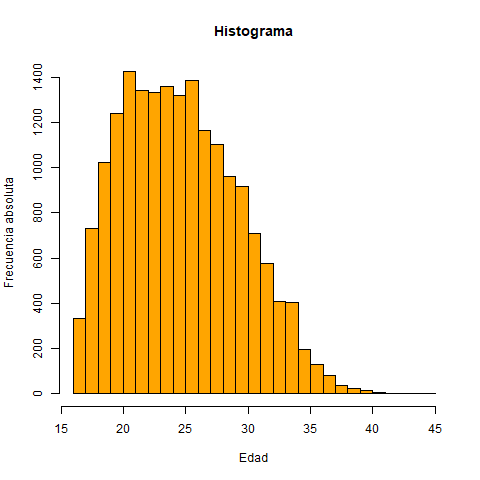
\includegraphics[width=\textwidth]{hist}


\bigskip
Procedemos a la separaci\'on de la variable en \textbf{clases de equivalencia} para calcular de ellas los distintos tipos de
frecuencia estudidados. Esto se hace gracias al uso de la librer\'ia \textbf{fdth} y para poder utilizarla, como se ha dicho 
anteriormente es necesario realizar lo siguiente:
\begin{Schunk}
\begin{Sinput}
> install.packages("fdth")
> library("fdth")
\end{Sinput}
\end{Schunk}

Procedemos al c\'alculo en s\'i:
\begin{Schunk}
\begin{Sinput}
> dist <- fdt(edad,breaks="Sturges")
> dist
\end{Sinput}
\begin{Soutput}
 Class limits    f   rf rf(%)    cf  cf(%)
      [16,18)  331 0.02  1.82   331   1.82
      [18,20) 1756 0.10  9.64  2087  11.46
      [20,21) 2663 0.15 14.63  4750  26.09
      [21,23) 2672 0.15 14.68  7422  40.76
      [23,25) 2677 0.15 14.70 10099  55.47
      [25,27) 1387 0.08  7.62 11486  63.09
      [27,29) 2263 0.12 12.43 13749  75.51
      [29,31) 1876 0.10 10.30 15625  85.82
      [31,32) 1281 0.07  7.04 16906  92.85
      [32,34)  812 0.04  4.46 17718  97.31
      [34,36)  323 0.02  1.77 18041  99.09
      [36,38)  119 0.01  0.65 18160  99.74
      [38,40)   25 0.00  0.14 18185  99.88
      [40,42)   18 0.00  0.10 18203  99.98
      [42,44)    1 0.00  0.01 18204  99.98
      [44,45)    3 0.00  0.02 18207 100.00
\end{Soutput}
\end{Schunk}

\begin{itemize}
\item Frecuencia absoluta -> f
\item Frecuencia relativa -> rf
\item Frecuencia relativa porcentual -> rf(\%)
\item Frecuencia abs acumulada -> cf
\item Frecuencia rel acumulada porcentual -> cf(\%)
\end{itemize}

\bigskip
Para calcular la \textbf{media} de edad hemos construido una funci\'on en R la cual es:
\begin{Schunk}
\begin{Sinput}
> source("media.R")
> media
\end{Sinput}
\begin{Soutput}
function(var) {
    sum<-0

    for (data in var) {
        sum<-sum+data
    }

    return(sum/length(var))
}
\end{Soutput}
\end{Schunk}

\bigskip
Procedemos al c\'alculo de la media haciendo uso de la misma:
\begin{Schunk}
\begin{Sinput}
> mf<-media(fifa$Age)
> mf
\end{Sinput}
\begin{Soutput}
[1] 25.12221
\end{Soutput}
\end{Schunk}

\bigskip
En cuanto a los \textbf{cuantiles}, para su visualizaci\'on hemos optado por el uso
de un diagrama de bigotes, donde adem\'as aparecen representados los l\'imites inferior
y superior de la variable de estudio. Para su realizaci\'on se ha hecho lo mismo que con el 
histograma de la siguiente manera:
\begin{Schunk}
\begin{Sinput}
> source("bigotes.R")
> bigotes
\end{Sinput}
\begin{Soutput}
function(var,ruta) {
    png(ruta)
 
    boxplot(var, col='green', horizontal=T) 

    dev.off()
}
\end{Soutput}
\end{Schunk}

\begin{Schunk}
\begin{Sinput}
> b<-bigotes(edad,"./bigotes.png")
\end{Sinput}
\end{Schunk}
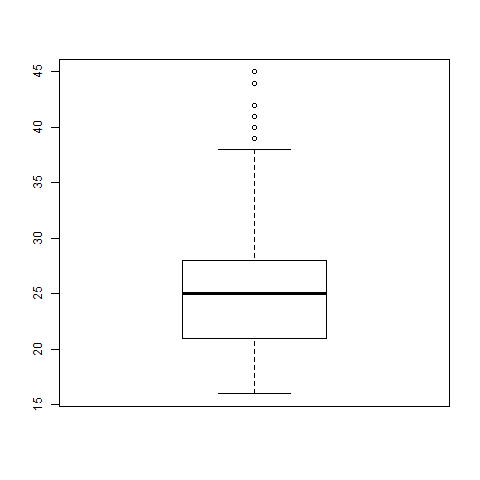
\includegraphics[width=\textwidth]{bigotes}

Para calcular la \textbf{desviaci\'on t\'ipica} hemos construido una funci\'on de la siguiente
forma:
\begin{Schunk}
\begin{Sinput}
> source("desviacion.R")
> desviacion
\end{Sinput}
\begin{Soutput}
function(var,media) {
    num<-0
    for (data in var){
        num<-num+((data-media)^2)
    }

    s<-sqrt(num/length(var))

    return(s)
}
\end{Soutput}
\end{Schunk}

El c\'alculo de la misma es:
\begin{Schunk}
\begin{Sinput}
> s<-desviacion(edad,mf)
> s
\end{Sinput}
\begin{Soutput}
[1] 4.669814
\end{Soutput}
\end{Schunk}

\bigskip
De acuerdo al teorema de \textit{Tchebychev} (realizado en una funci\'on aparte) el intervalo en el que se encuentran el 75\%
de los datos, es decir para k=2, es:
\begin{Schunk}
\begin{Sinput}
> source("tche.R")
> t<-tche(s,mf,2)
> toString(t)
\end{Sinput}
\begin{Soutput}
[1] "15, 34"
\end{Soutput}
\end{Schunk}

Dicha funci\'on es:
\begin{Schunk}
\begin{Sinput}
> tche
\end{Sinput}
\begin{Soutput}
function(des,media,k) {
    
    rango<-des*k
    inter<-list(as.integer(media-rango),as.integer(media+rango))

    return(inter)
}
\end{Soutput}
\end{Schunk}

Observando el intervalo tan amplio necesario para englobar el 75\% de los datos se puede concluir con que la media
no es una buena medida representante del conjunto de datos estudiado.

\bigskip
El c\'alculo de la \textbf{varianza} es sencillo, \'unicamente es la desviaci\'on al cuadrado:
\begin{Schunk}
\begin{Sinput}
> v<-s^2
> v
\end{Sinput}
\begin{Soutput}
[1] 21.80717
\end{Soutput}
\end{Schunk}

\end{document}
